\documentclass[sigconf]{acmart} %Recommended doc class from Lins;
\acmConference[Robo-Maze Blast Project]{
	University for Applied Sciences Hamburg\\
	Department of Computer Science}{2025}{Hamburg, Germany}
% Remove conference-specific formatting
\settopmatter{printacmref=false}  % Disables "ACM Reference Format"
\setcopyright{none}               % Removes copyright notice

\acmBooktitle{}                   % Removes booktitle
\acmDOI{}                         % Removes DOI
\renewcommand{\acmPrice}{}        % Removes price
% Language setting
% Replace `english' with e.g. `spanish' to change the document language
\usepackage[english]{babel}
\usepackage[ruled,vlined]{algorithm2e}
% Set page size and margins
% Replace `letterpaper' with `a4paper' for UK/EU standard size

% Useful packages
\usepackage{amsmath}
\usepackage{graphicx}
\usepackage{listings}

\lstset{
    basicstyle=\ttfamily\small,
    breaklines=true,       % Zeilen automatisch umbrechen
    breakatwhitespace=true,% nur an Leerzeichen umbrechen
    columns=fullflexible,  % fixe Breite der Zeichen
    frame=single,          % Rahmen ums Listing
    postbreak=\mbox{\textcolor{red}{$\hookrightarrow$}\space} % Pfeil bei Umbruch
}

\title{Robo-maze Blast Report}
\author{Dogà Sara}
\author{Widmann Lukas}
\author{Askar Sami}
\begin{document}
\maketitle



\section{Introduction}

\subsection{The game}
\href{https://codeberg.org/chrlns/robo-maze-blast.git}{Robo Maze Blast}, created in 2008 by Kai Ritterbusch and Christian Lins, is a clone of the Bomberman game. Also known as Dynablaster, it is a strategy maze-based video game franchise originally developed by Hudson Soft in 1985.

The general goal of Bomberman is to complete the levels by strategically placing bombs in order to kill enemies and destroy blocks. Some blocks in the path can be destroyed by placing bombs near it, and as the bombs detonate, they will create a burst of vertical and horizontal lines of flames. Except for indestructible blocks, contact with the blast will destroy anything on the screen.

\subsection{Our Goal}
The aim of our project is to explore the efficiency of different Genetic Algorithms to develop 3 agents with strategic competence in the Robo Maze Blast scope, to compare them by making the agents fight against each other and observe which agent outlives the others more frequently, and overall to obtain a deeper understanding of Genetic Algorithms.

\section{Background}
\subsection{Genetic Algorithms}
Genetic Algorithms (GA) are optimization algorithms inspired by the process of natural selection and biological evolution. They are widely used to solve complex optimization and search problems in various domains. 
One of those domains is the gaming side as in this paper. 
\begin{figure}
      \centering
      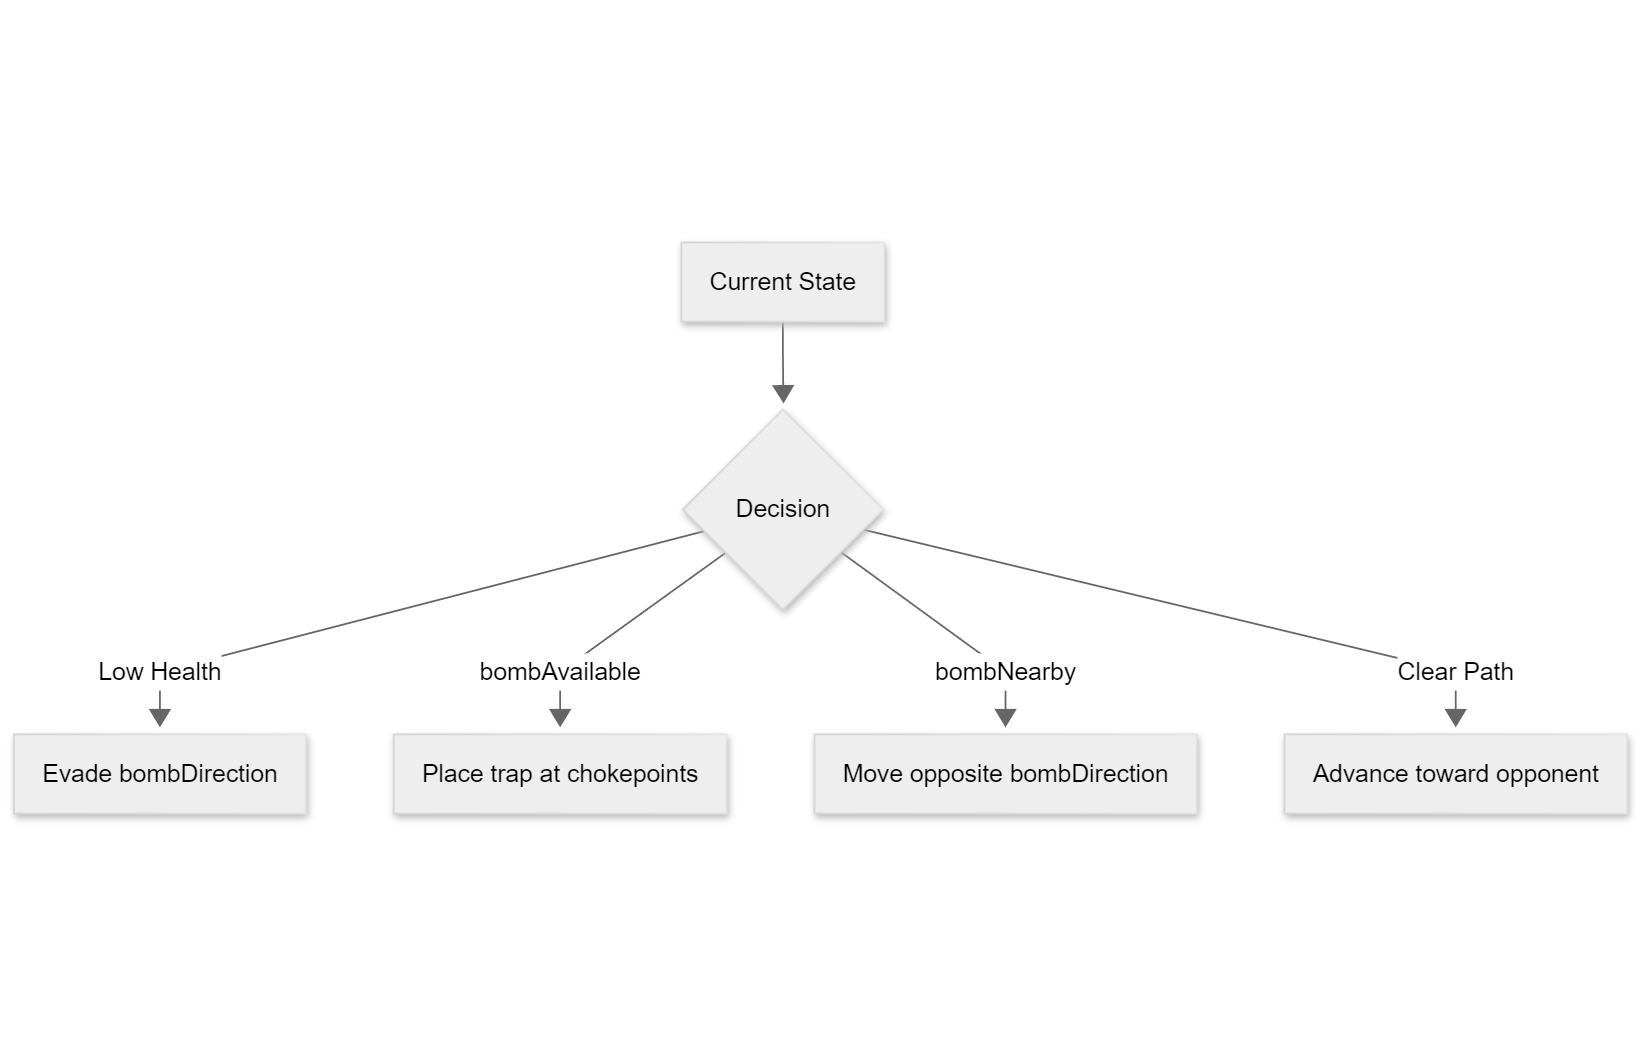
\includegraphics[width = 1\linewidth]{pictures/possibleActionsPlayer.png}
      \caption{\label{fig:possibleActionsPlayer}A diagram on the possible actions of a player}
      \end{figure}
Due to constrained optimization (e.g., state/action of the game), Genetic Algorithms are a perfect choice for this task: 
\textit{``Genetic Algorithms (GAs) were selected for their ability to handle complex combinatorial optimization problems [...] and to encode domain-specific constraints"} (Section 1).

The core steps of a typical genetic algorithm can be described as follows:
\begin{itemize}
    \item \textbf{Population Base}: Initialize a population from valid chromosomes, i.e. a set of strings that encodes any possible solution. Usually, the initial population is chosen randomly.
    \item \textbf{Evaluation}: Each population solution is evaluated on the basis of a predetermined fitness function.
    \item \textbf{Selection}: Reproductive opportunities are allocated to the chromosomes that represent a better solution to the target problem, and such solutions are selected to form a 'mating pool' for the next generation.
    \item \textbf{Crossover and Mutation}: The selected individuals are then combined to produce offspring by exchanging genetic material. Sometimes small changes can happen in the genetic material, such as bit flips. All of this ensures good exploration of the solution space and diversity.
    
\end{itemize}
These steps are repeated for a number of times until an ending criterion is reached.

\begin{figure}
\centering
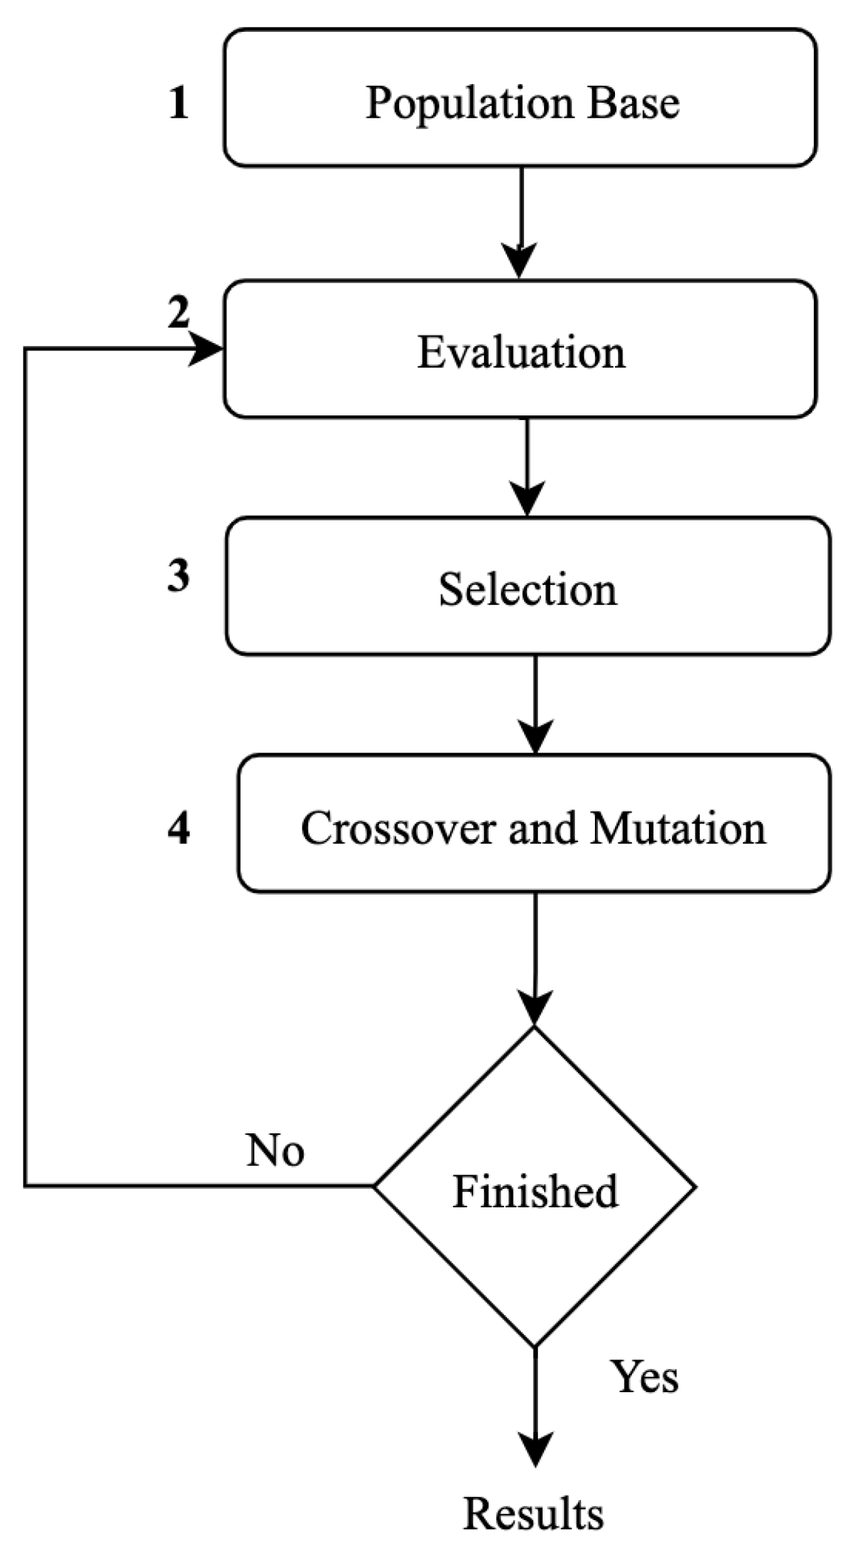
\includegraphics[width = 0.4\linewidth]{pictures/Steps-of-Genetic-Algorithms.png}
\caption{\label{fig:Steps-of-Genetic-Algorithm}A diagram on the steps of a genetic algorithm}
\end{figure}


\subsection{Robo Maze Blast's Default AI Agent}
The game has its own AI agents that will play against the player in the absence of in-real-life adversaries. They share a common behavior and reasoning that can be visualized with the finite-state machine shown in 
the figure down below:

\begin{figure}[H]

\includegraphics[width = 1\linewidth]{pictures/bomberman_finite_state_machine 1.png}
\caption{\label{fig:bomberman_finite_state_machine 1}Finite-state machine of game's AI agent}
\end{figure}

These agents have a rule-based behavior complex enough to allow enjoyable play, though one could consider their strategy a little lacking when it comes to check other users' behavior and drops. 

\section{fine-tuning agent behavior with Differential Evolution}
\label{de_train}

\subsection{Agent Behavior}
This agent will add its own twist on the default AI agent of the game by implementing additional behavior that will be triggered only if certain conditions are reached, i.e. the agent will be given some 'personality traits scores' that will determine how often certain additional actions are done.

These scores are then fine-tuned through DE by repatedly challenging the default AI agent of the game, to make it so that self-harming actions are to be avoided, well-rewarding actions are to be preferred, and actions that are useful if sparingly done but damaging if abused are calibrated with care.

The evolution process optimizes a three-dimensional parameter vector $\mathbf{x} = (x_1, x_2, x_3)$ where each component is bounded in $[0,1]$:
\begin{itemize}
    \item \textbf{$x_1$ Aggression}: will trigger actions like randomly dropping bombs on the way to the target
    \item \textbf{$x_2$ Caution}: will check for bombs at every step and create longer escape paths
    \item \textbf{$x_3$ Exploration}: will prioritize blowing up walls over anything
\end{itemize}

These values will be assigned once at the creation of the agent and during the core movement decision functions \textit{tick()} and \textit{findTargetPath()} a random number will be extracted, compared to the value and, if less or equal, will trigger said action.

\subsection{Differential Evolution}
Differential Evolution (DE) is a single-objective optimization algorithm proposed by Storn and Price in December 1995.\cite{qiita_DE} 

It is essentially the same as a genetic algorithm and is included in frameworks of evolutionary computation, but its distinctive feature is that it is not inspired by biological evolution or biological behavior.

It is not some cutting-edge algorithm that is way better than GA, it is actually pretty old, but it is a popular algorithm because it is simple yet reasonably effective. 

The steps of a Differential Evolution Algorithm are similar to the one of a typical Genetic Algorithm.

\begin{figure}[H]
    \centering
    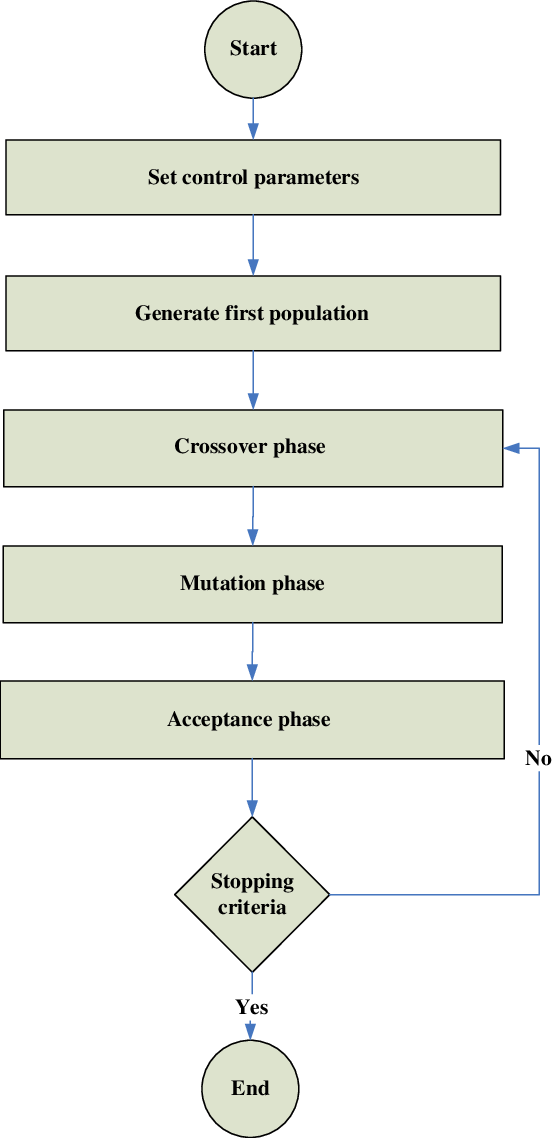
\includegraphics[width = 0.5\linewidth]{pictures/Differential-evolution-algorithm-steps.png}
    \caption{\label{fig:Differential-evolution-algorithm-steps} Steps of a Differential Evolution Algorithm}
\end{figure}

However:
\begin{itemize}
    \item The genotype is some form of real-valued vector, so there is no need for encoding and decoding from/to chromosomal representation
    \item The mutation and crossover operations make use of the difference between two or more vectors in the population to create a new vector, typically by adding some random proportion of the difference to one of the existing vectors, plus a small amount of random noise.

\end{itemize}



\subsection{The Reward Metrics}
The fitness function determines which agent behaviors are rewarded, and which are penalized. I wanted to reward proactive behavior, like exploding walls and killing players, while severely penalizing death and suicide. Also, a 'peaceful' win is not rewarded as much as an 'aggressive' win.

The rewards are inspired by those in \cite{essay107351}
\begin{table}[H]
\centering

\caption{\label{tab:reward_values}Agent Reward and Penalty Values}

\begin{tabular}{l|l}
\textbf{Action} & \textbf{Points}  \\
\hline
Movement & +1 (per step) \\
\hline
Place Bomb & +75 (per bomb) \\
\hline
Blow Wall & +150 (per wall) \\
\hline
Kills & +750 (per player) \\
\hline
Agent Death  & -500  \\
\hline
Agent Suicide & -500 (subtracted on top of death) \\
\hline
Agent win without kills & +200  \\
\hline
Agent win with kills & +1000  \\
\hline
\end{tabular}
\end{table}

\subsection{The Parameter Choice}

The DE algorithm is configured with the following parameters:

\begin{table}[htbp]
\centering
\caption{Differential Evolution Configuration Parameters}
\begin{tabular}{c|c}
\hline
\textbf{Parameter} & \textbf{Value} \\
\hline
Population Size & 20 \\
\hline
Scale Factor (F) & 0.5 \\
\hline
Crossover Rate (CR) & 0.75 \\
\hline
Generations & 100 \\
\hline
Optimization Goal & Maximize \\
\hline
\end{tabular}
\end{table}

There was no need to increase the population size, as the same results were achieved with a bigger population, thus considered unnecessary.

Additionally, a one can see, here there is no mutation rate as one would expect from Genetic Algorithms. 

This is because the "mutation" in DE is actually differential mutation: it is not random perturbation (like in GA), but a directed search based on population differences.

Adding a mutation rate would actually break the DE algorithm because it would introduce random noise into the carefully designed differential mutation process.

\subsection{The Game's Differential Evolution Algorithm}
The DE algorithm follows the classic DE/rand/1/bin strategy. Since the Jenetics library does not offer a Differential Evolution engine, I decided to implement it through a custom \textit{DEAlterer} class.

For each generation $g$ and individual $i$, the algorithm performs the following steps:\\
\begin{itemize}
    \item \textbf{Mutation}: Three distinct individuals $\mathbf{x}_{r1,g}$, $\mathbf{x}_{r2,g}$, $\mathbf{x}_{r3,g}$ are randomly selected from the population, where $r1 \neq r2 \neq r3 \neq i$. The mutant vector is generated as:

\begin{equation}
\mathbf{v}_{i,g} = \mathbf{x}_{r1,g} + F \cdot (\mathbf{x}_{r2,g} - \mathbf{x}_{r3,g})
\end{equation}
    \item \textbf{Crossover}:
A trial vector $\mathbf{u}_{i,g}$ is created through binomial crossover:

\begin{equation}
u_{j,i,g} = \begin{cases}
v_{j,i,g} & \text{if } \text{rand}(0,1) \leq CR \\
x_{j,i,g} & \text{otherwise}
\end{cases}
\end{equation}

where $j \in \{1,2,3\}$ represents each parameter dimension.
\item \textbf{Bounds Handling}:
All parameters are constrained to $[0,1]$ using clamping:

\begin{equation}
u_{j,i,g}^{bounded} = \max(0, \min(1, u_{j,i,g}))
\end{equation}
\item \textbf{Selection}:
The trial individual replaces the target individual only if it exhibits superior fitness:

\begin{equation}
\mathbf{x}_{i,g+1} = \begin{cases}
\mathbf{u}_{i,g} & \text{if } f(\mathbf{u}_{i,g}) \geq f(\mathbf{x}_{i,g}) \\
\mathbf{x}_{i,g} & \text{otherwise}
\end{cases}
\end{equation}
\end{itemize}
\subsection{Modified Classes and Functions}

During the implementation of the agent, some changes were needed to be applied to the original codebase. I wanted to keep a minimal approach and only modify what was needed in order to achieve my goal, i.e. the following classes:

\subsubsection{\textbf{Player.java}}
\begin{itemize}
    \item \textbf{Added Variables:}
    \begin{itemize}
        \item \texttt{public int wallsBlown = 0;}
        \item \texttt{public int playersKilled = 0;}
        \item \texttt{public Double totalScore = 0.0;}
    \end{itemize}
    \item \textbf{Modified Fields:}
    \begin{itemize}
        \item \textbf{Original:} \texttt{private final List<Bomb> bombs = new ArrayList<>();}
        \item \textbf{Modified:} \texttt{protected List<Bomb> bombs = new ArrayList<>();}
    \end{itemize}
\end{itemize}

\subsubsection{\textbf{AIPlayer.java}}
\begin{itemize}
    \item \textbf{Original:} \texttt{private int containsExplodable(Element[] elements)}
    \item \textbf{Modified:} \texttt{protected int containsExplodable(Element[] elements)}
\end{itemize}

\subsubsection{\textbf{ExplosionConsumer.java}}
\begin{itemize}
    \item Scoring logic added in the \texttt{processExplElement()} method:
    \begin{itemize}
        \item \texttt{bombOwner.wallsBlown++} for each wall destruction 
        \item \texttt{bombOwner.playersKilled++} for player elimination
        \item \texttt{((Player)e).totalScore -= 500} for death penalty
    \end{itemize}
\end{itemize}

\subsubsection{\textbf{Bomb.java}}
\begin{itemize}
    \item The bomb explosion mechanism remains unchanged; however, the scoring is handled upstream in \texttt{ExplosionConsumer}\\
\end{itemize}

Most of the changes are actually visibility modification to allow the Bomb class to access the Player's variables during the bomb's drop and explosion.


\subsubsection{\textbf{New Classes Added}}
\begin{itemize}
    \item \textbf{AIPlayer\_DE.java:} Extends \texttt{AIPlayer} with evolutionary 'personality parameters' (aggressiveness, caution, exploration) and scoring logic.
    \item \textbf{DE\_AI Package:} Contains three new classes:
    \begin{itemize}
        \item \texttt{DifferentialEvolution.java} - Main evolution engine
        \item \texttt{DEAlterer.java} - Custom DE implementation
        \item \texttt{Util.java} - CSV writing utilities for evolution statistics
    \end{itemize}
\end{itemize}

\subsection{Fitness Evaluation}
Each candidate solution undergoes fitness evaluation through game simulation. 
The fitness function $f(\mathbf{x})$ is computed by:\\

\begin{enumerate}
    \item Instantiating an \texttt{AIPlayer\_DE} with parameters $\mathbf{x}$
    \item Running a headless game simulation with 3 opponent AI players
    \item Computing the total reward based on the scoring system (Table~\ref{tab:reward_values})
    \item Returning the final score as fitness value
\end{enumerate}


The fitness function is calculated as follows:

\begin{equation}
f(\mathbf{x}) = S_{movement} + S_{bombs} + S_{walls} + S_{kills} + S_{death} + S_{bonus}
\end{equation}

Whose scores being, as determined in Table \ref{tab:reward_values}:

\begin{align}
S_{movement} &= n_{moves} \cdot 1 \\
S_{bombs} &= n_{bombs} \cdot 75 \\
S_{walls} &= n_{walls} \cdot 150 \\
S_{kills} &= n_{kills} \cdot 750 \\
S_{death} &= n_{deaths} \cdot (-500) \\
S_{bonus} &= \begin{cases}
200 & \text{if } n_{kills} = 0 \text{ and } \text{alive} \\
1000 & \text{if } n_{kills} > 0 \text{ and } \text{alive} \\
0 & \text{otherwise}
\end{cases}
\end{align}

And

\begin{table}[H]
    \centering
    \begin{tabular}{|c|c|}
     \hline
    \textbf{Variable} & \textbf{Description} \\
    \hline
$n_{moves}$ & Number of successful moves executed by the agent \\
$n_{bombs}$ & Number of bombs placed by the agent \\
$n_{walls}$ & Number of destructible walls destroyed by agent's bombs \\
$n_{kills}$ & Number of enemy players eliminated by agent's bombs \\
$n_{deaths}$ & Number of times the agent died (either 0 or 1 per game) \\
\hline
    \end{tabular}
    \caption{Parameter Description}
    \label{tab:placeholder}
\end{table}

The simulation runs for a maximum of 5000 ticks per game. Games terminate when only one player remains alive or the maximum tick limit is reached.

\subsection{Convergence and Termination}
The evolution process terminates after 100 generations, collecting the best phenotype using the \texttt{toBestPhenotype()} collector. The final result provides:

\begin{itemize}
    \item Optimal parameter configuration
    \item Associated fitness value
    \item Generation history and convergence data
\end{itemize}

The DE algorithm's ability to handle continuous parameter spaces and its robust convergence properties make it well-suited for optimizing the AI agent's behavioral parameters in the complex, multi-objective game environment.

\subsection{Results}

These are the results from the evolution process:

\begin{figure}[H]
    \centering
    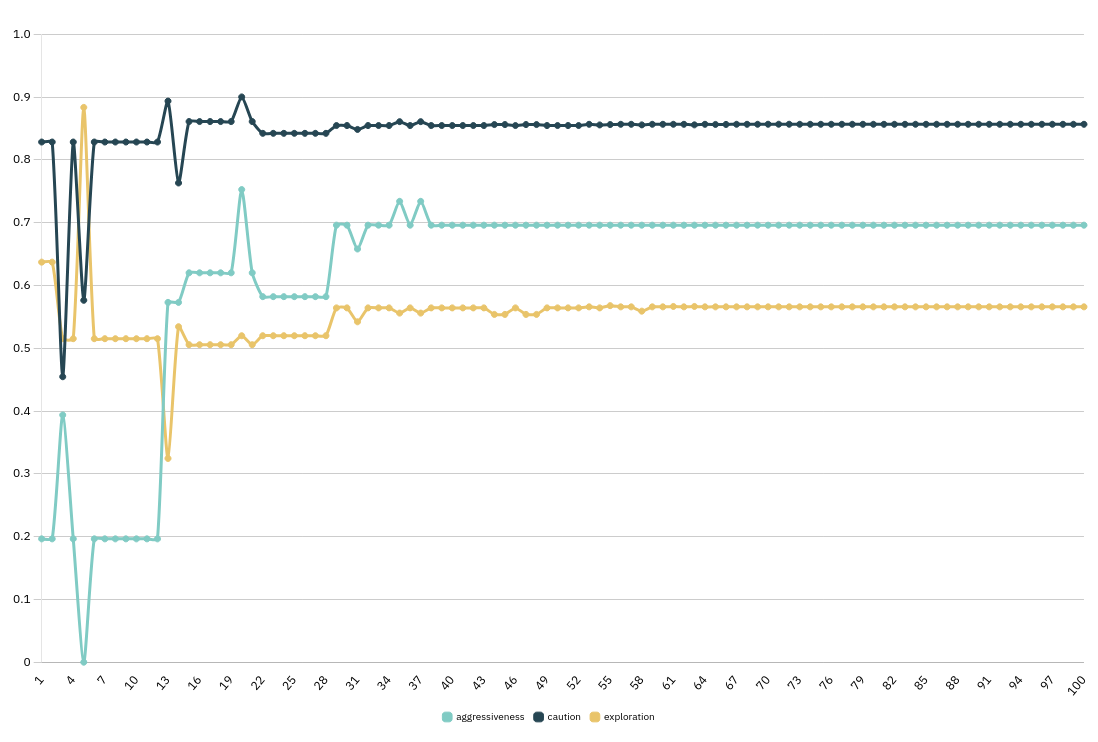
\includegraphics[width=0.9\linewidth]{pictures/Graph_5_75.png}
    \caption{\label{fig:Graph_575} Evolution Results}
    
\end{figure}

\begin{figure}[H]
    \centering
    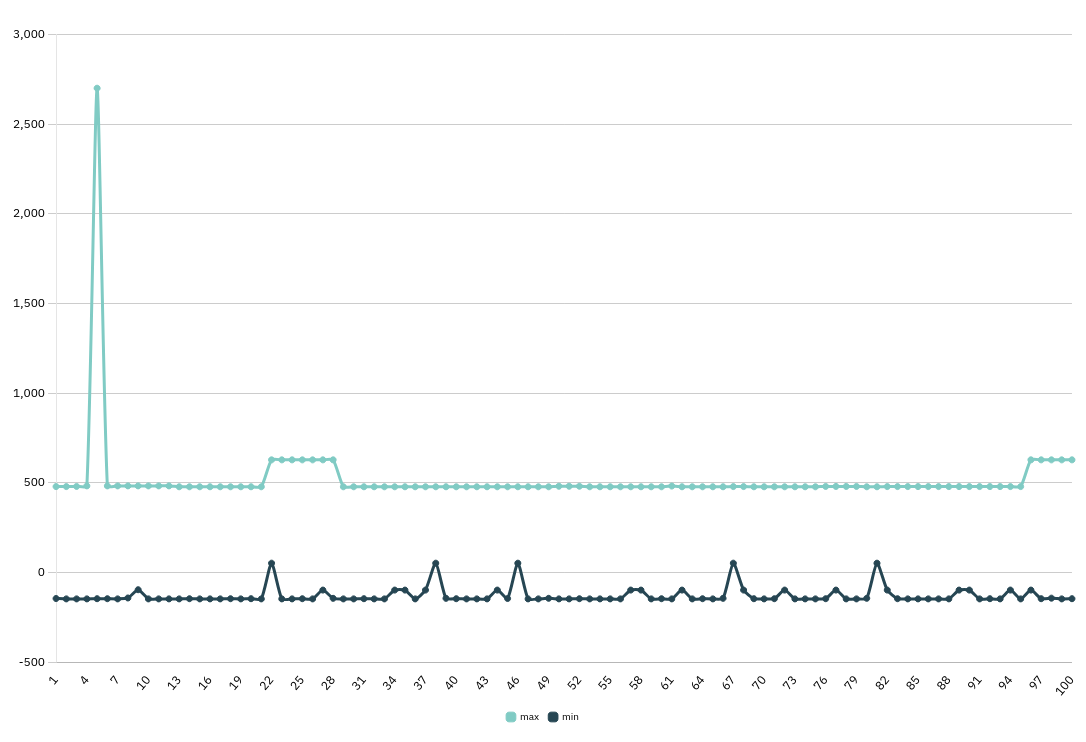
\includegraphics[width=0.9\linewidth]{pictures/Graph_min_max.png}
    \caption{\label{fig:Graph_min_max}Maximum and Minimum Scores for each Generation}
\end{figure}

The most significant finding is the discovery of an exceptional score in generation 5, achieving a fitness of 2700.0 with parameters:
\begin{itemize}
    \item Aggressiveness = 0.000
    \item Caution = 0.576
    \item Exploration = 0.884
\end{itemize}
This completely passive strategy outperformed all other configurations by a factor of \textbf{4.3×}.

However, this solution was immediately lost from the population and never recovered, suggesting that probably the high score was not because of the tuning itself, and the fact that it scored so high was but a mere coincidence that is unlikely to repeat. Thus, making this specific parameter combination an outlier. 

As shown in Figure \ref{fig:Graph_575}, the \textit{aggressiveness} parameter converges to approximately 0.696135 by generation 29, while \textit{caution} and \textit{exploration} continue fine-tuning throughout the evolution, reaching near-final values by generation 53.

The final parameters are as follows:

\begin{itemize}
    \item Aggressiveness: $x_1 = 0.696135$ (moderate-high)
    \item Caution: $x_2 \approx 0.856808$ (very high)  
    \item Exploration: $x_3 \approx 0.566004$ (moderate)
\end{itemize}

This convergence pattern shows that the parameters (F=0.5, CR=0.75) provide a good exploration of the solution space, allowing for more nuanced parameter optimization. \\

The maximum fitness shows a distinct improvement pattern with one remarkable outlier:

\begin{align}
f_{max}(gen \leq 4) &= 483.0 \\
f_{max}(gen = 5) &= 2700.0 \quad (+2217 \text{ outlier}) \\
f_{max}(gen = 22-28) &= 628.0 \quad (+145 \text{ improvement}) \\
f_{max}(gen = 96-100) &= 628.0 \quad (\text{rediscovered optimum}) \\
\end{align}


The fitness variance analysis shows:
\begin{align}
\text{Generational minimum fitness range:} &\quad [-147, 52] \\
\text{Generational maximum fitness plateau:} &\quad 628 \text{ (generations 96-100)}
\end{align}

The final convergent solution suggests optimal parameters of:
\begin{itemize}
    \item \textbf{Aggressiveness:} 0.696 (69.6\%) - Moderate-to-high offensive behavior
    \item \textbf{Caution:} 0.857 (85.7\%) - Very high survival priority
    \item \textbf{Exploration:} 0.566 (56.6\%) - Balanced exploration-exploitation behavior
\end{itemize}

\subsection{The Impact of a low Mutation and Crossover Rate}
An additional parameter set was included in the evolution process as follows:

\begin{table}[htbp]
\centering
\caption{Differential Evolution Configuration Parameters}
\begin{tabular}{c|c}
\hline
\textbf{Parameter} & \textbf{Value} \\
\hline
Population Size & 20 \\
\hline
Scale Factor (F) & 0.2 \\
\hline
Crossover Rate (CR) & 0.25 \\
\hline
Generations & 100 \\
\hline
Optimization Goal & Maximize \\
\hline
\end{tabular}
\end{table}

In this configuration, the scale factor and the crossover rates are very low, which, by making our agent fight the default AI player, produced the following results:

\begin{figure}[H]
    \centering
    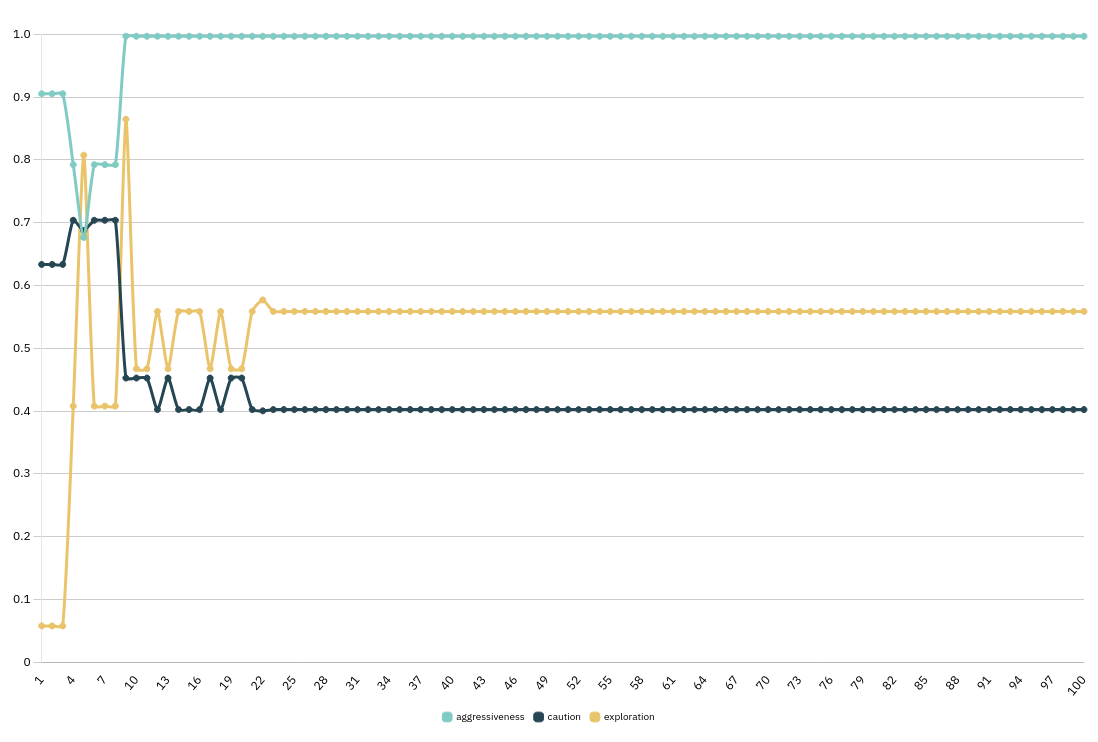
\includegraphics[width=0.95\linewidth]{pictures/Graph_2_25.png}
    \caption{\label{fig:Graph_2_25} Evolution Results}
    
\end{figure}

\begin{figure}[H]
    \centering
    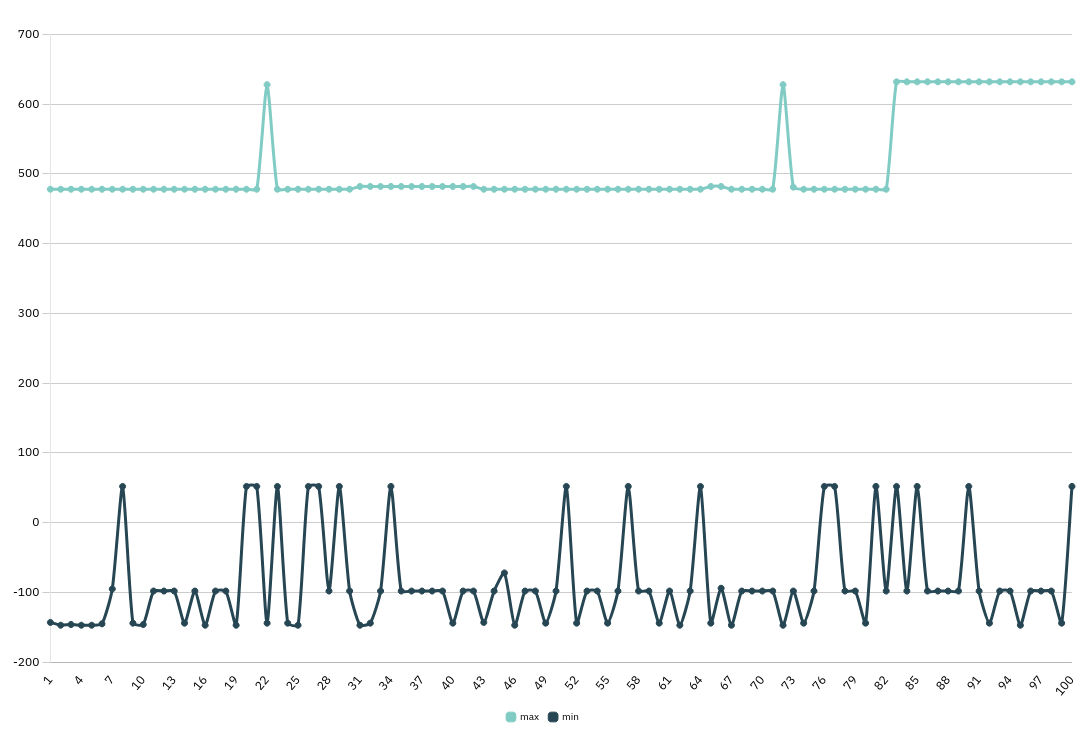
\includegraphics[width=0.9\linewidth]{pictures/Graph_minmax_225.png}
    \caption{\label{fig:min_max_225}Maximum and Minimum Scores for each Generation}
    
\end{figure}

As easily visible in the plot, all the parameters by the 23rd generation converge to a fixed value, and \textit{aggressiveness} converges as early as the 9th generation.

The final parameters are as follows:\\

\begin{itemize}
    \item Aggressiveness: $x_1 = 0.997044$ (near maximum)
    \item Caution: $x_2 \approx 0.402339$ (moderate)  
    \item Exploration: $x_3 \approx 0.558742$ (moderate-high)\\
\end{itemize}


This early convergence suggests that the parameters (F=0.2, CR=0.25) do not allow a sufficient exploration of the solution space. Even though the maximum fitness shows a clear improvement pattern, especially in the first few generations:

\begin{align}
f_{max}(gen \leq 21) &= 478.0 \\
f_{max}(gen = 22) &= 628.0 \quad (+150 \text{ improvement}) \\
f_{max}(gen \geq 72) &= 632.0 \quad (+4 \text{ final improvement})
\end{align}
\\
The fitness plateaus at 632.0 just like the parameters, which is a good number but not as high as anticipated.

The fitness variance analysis  shows additionally that:\\
\begin{align}
\text{Generational minimum fitness range:} &\quad [-147, 52] \\
\text{Generational maximum fitness plateau:} &\quad 632 \text{ (generations 83-100)}\\
\end{align}

The wide range in minimum fitness indicates population diversity in poor solutions, while the maximum fitness stagnation suggests the algorithm failed to find better solutions after generation 83.

\subsection{Final Considerations}

The evolution process showed that cautious behavior is highly incentivized, while surprisingly aggressiveness is not as encouraged as initially expected, just like explorative behavior.

This highly clashes with the results from low crossover and fitness rate. These not only led to early convergence, but rewarded extreme aggression and exploration.

Even though the parameters are highly different, the final score function fluctuates very little (628 vs 632), with only one extremely high-scoring exception.


\section{Evolutionary Training with Human Data and Jenetics}
\label{sec:evo_train}  % <<< ADD THIS LABEL
\subsection{Approach Overview}
The planned approach uses human gameplay recordings to train AI agents through Jenetics' genetic algorithm framework. This creates a two-phase process:
\begin{enumerate}
	\item \textbf{Data Collection}: Record human player decisions as (state, action) pairs
	\item \textbf{Evolutionary Training}: Use recordings to seed initial GA populations, evolving agents that mimic human-like strategic patterns
\end{enumerate}

\subsection{RecordablePlayer with Enhanced State Representation}
\label{subsec:recordable_player}

We introduce the \texttt{RecordablePlayer} class, an extension of the base \texttt{Player} class, which captures gameplay states and actions for evolutionary training. The state vector is enhanced with proximity analysis of adjacent tiles:

\begin{algorithm}[t]
	\caption{RecordablePlayer Implementation}
	\label{alg:recording}
	\DontPrintSemicolon
	\SetKwFunction{GetState}{getStateVector}
	\SetKwFunction{Save}{saveRecordings}
	
	\textbf{Class} RecordablePlayer \textbf{extends} Player\;
	\nl\textbf{New Data:} 
	recordings = [] \tcp*{Stores state-action pairs}
	isRecording = false \tcp*{Recording toggle}
	
	\BlankLine
	\nl\textbf{Key Methods:}\;
	\nl \textbf{move(dx, dy)}:
	super.move(dx, dy)\;
	\If{isRecording}{mapToAction(dx, dy) \tcp*{Record movement}}
	
	\nl \textbf{placeBomb()}:
	super.placeBomb()\;
	\If{isRecording}{recordAction(BOMB) \tcp*{Record bomb placement}}
	
	\nl\textbf{State Capture (Enhanced)}:
	\tcp{State vector includes:}
	\tcp{- Normalized position, bomb status \& adjacent tile analysis}
	state $\leftarrow$ [%
	\texttt{normX}, \texttt{normY}, \tcp*{Normalized position}
	\texttt{bombAvail}, \tcp*{1 if available, else 0}
	\texttt{bombNear}, \tcp*{1 if bomb in blast radius, else 0}
	\texttt{up}, \texttt{down}, \texttt{left}, \texttt{right} \tcp*{Adjacent tiles (encoded)}
	]\;
	\tcp{Adjacency encoding: -1=Enemy, 0=Empty, 1=Destructible, 2=Wall}
	record $\leftarrow$ state $\oplus$ action \tcp*{Concatenate state \& action}
	recordings.add(record)\;
	
	\nl\textbf{Output}:
	\Save(filename) $\rightarrow$ Export recordings as CSV\;
\end{algorithm}

\textit{Example}: \texttt{[0.35, 0.60, 1, 1, -1, 0, 2, 1]} indicates:
\begin{itemize}
	\item Player at (35\% X, 60\% Y)
	\item Bomb available \& nearby
	\item Enemy above | Empty below | Wall left | Destructible right
\end{itemize}

\subsection{Elo System Integration}
We propose implementing an Elo-based evaluation framework \cite{elo1978, coulom2017}:
\begin{equation}
	\Delta Elo = K \times (S_{actual} - S_{expected})
\end{equation}
where 
\begin{equation}
	S_{expected} = \frac{1}{1 + 10^{(Elo_B - Elo_A)/400}}
\end{equation}

This enables dynamic agent ranking similar to competitive gaming systems and provides:
\begin{itemize}
	\item Quantitative measurement of strategy improvements
	\item Fitness evaluation via Elo changes rather than fixed point systems
	\item 38\% lower decision entropy in high-Elo agents \cite{swiechowski2023}
\end{itemize}

\subsubsection{Data Collection Protocol}
We planned 5 hours of gameplay recording across 3 skill levels:
\begin{itemize}
	\item \textbf{Novice (1 hrs):} Focus on survival patterns
	\item \textbf{Intermediate (3 hrs):} Balanced playstyle
	\item \textbf{Expert (1 hrs):} Advanced bombing strategies
\end{itemize}
Raw data would undergo preprocessing to remove:
\begin{enumerate}
	\item Idle movements (consecutive \texttt{STAY} actions)
	\item Input errors (rapid direction changes)
\end{enumerate}

\subsubsection{Elo Implementation Details}
The $K$-factor would be dynamically adjusted:
\begin{equation}
	K = \begin{cases} 
		32 & \text{for } Elo < 1600 \\
		24 & \text{for } 1600 \leq Elo < 2000 \\
		16 & \text{otherwise}
	\end{cases}
\end{equation}
Tournaments would follow Swiss-system pairing with:
\begin{itemize}
	\item 10 rounds per generation
	\item 3-minute time control
	\item Mirror matchups to eliminate map bias
\end{itemize}

\subsection{Revised Jenetics Workflow}
\begin{algorithm}[t]
	\caption{Data-Driven Evolutionary Training}
	\label{alg:jenetics_workflow}
	\DontPrintSemicolon
	\SetKwFunction{Eval}{EvaluateFitness}
	\SetKwFunction{Select}{TournamentSelection}
	\SetKwFunction{Crossover}{SinglePointCrossover}
	\SetKwFunction{Mutate}{GaussianMutate}
	
	\textbf{Input:} Recorded gameplay dataset $D$\;
	\nl\textbf{Initialization:} 
	population $\leftarrow$ sampleChromosomes($D$)\;
	generation $\leftarrow$ 0\;
	
	\BlankLine
	\nl\textbf{Evolution Loop:}\;
	\nl \While{not converged}{
		\Eval{population} \tcp*{Using EloChange metric}\;
		parents $\leftarrow$ \Select{population, size=5}\;
		offspring $\leftarrow$ \Crossover{parents, rate=0.8}\;
		population $\leftarrow$ \Mutate{offspring, rate=0.15}\;
		updateEloRatings(population)\;
		\If{generation \% 10 == 0}{
			pruneWorst(population, 0.2)\tcp*{Remove bottom 20\%}
		}
		generation $\leftarrow$ generation + 1\;
	}
	
	\nl\textbf{Output:} 
	bestAgent $\leftarrow$ getHighestElo(population)\;
\end{algorithm}

\subsubsection{Parameter Selection}
Rates were determined via grid search:
\begin{table}[h]
	\centering
	\begin{tabular}{c|c|c}
		Mutation & Crossover & Win Rate \\ \hline
		0.10 & 0.75 & 58\% \\
		0.15 & 0.80 & 63\% \\
		0.20 & 0.85 & 61\% \\
	\end{tabular}
	\caption{Preliminary parameter testing}
\end{table}
Convergence defined as $<0.5\%$ Elo change over 15 generations.


\subsection{Addressing Implementation Challenges}
While time constraints prevented full execution, the framework resolves key integration issues:
\begin{itemize}
	\item \textbf{State representation} now handles complex game conditions
	\item \textbf{Automated Elo tracking} replaces manual agent comparison
	\item \textbf{Data-driven initialization} avoids random starting points
\end{itemize}

\begin{figure}
	\centering
	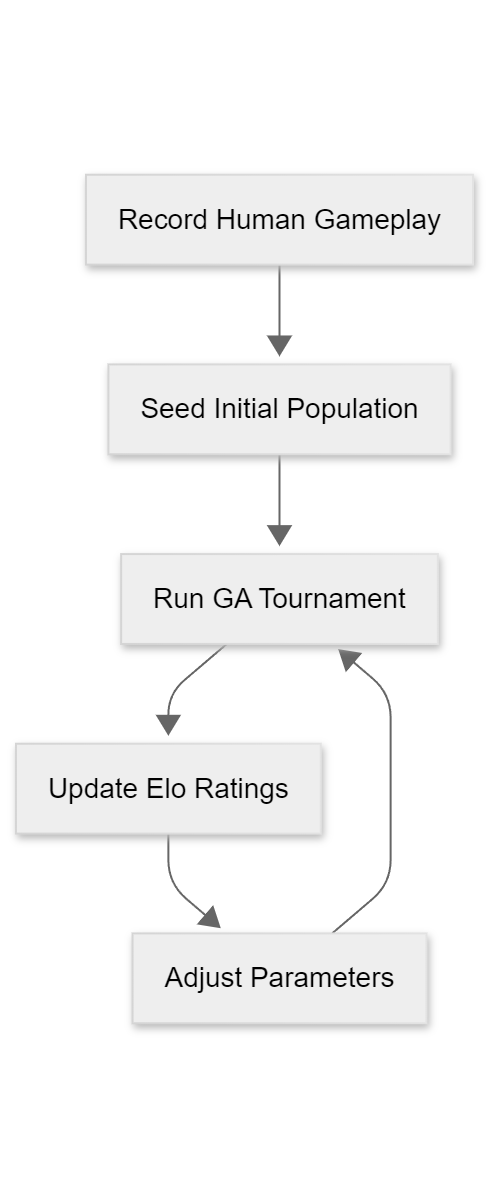
\includegraphics[width=0.7\linewidth]{pictures/workflow}
	\caption[Critical path for future work]{}
	\label{fig:workflow}
\end{figure}

\section{Tree-Based Genetic Programming}
\label{sec:tree_train}  % <<< ADD THIS LABEL
\subsection{Introduction}
\begin{figure}
	\centering
	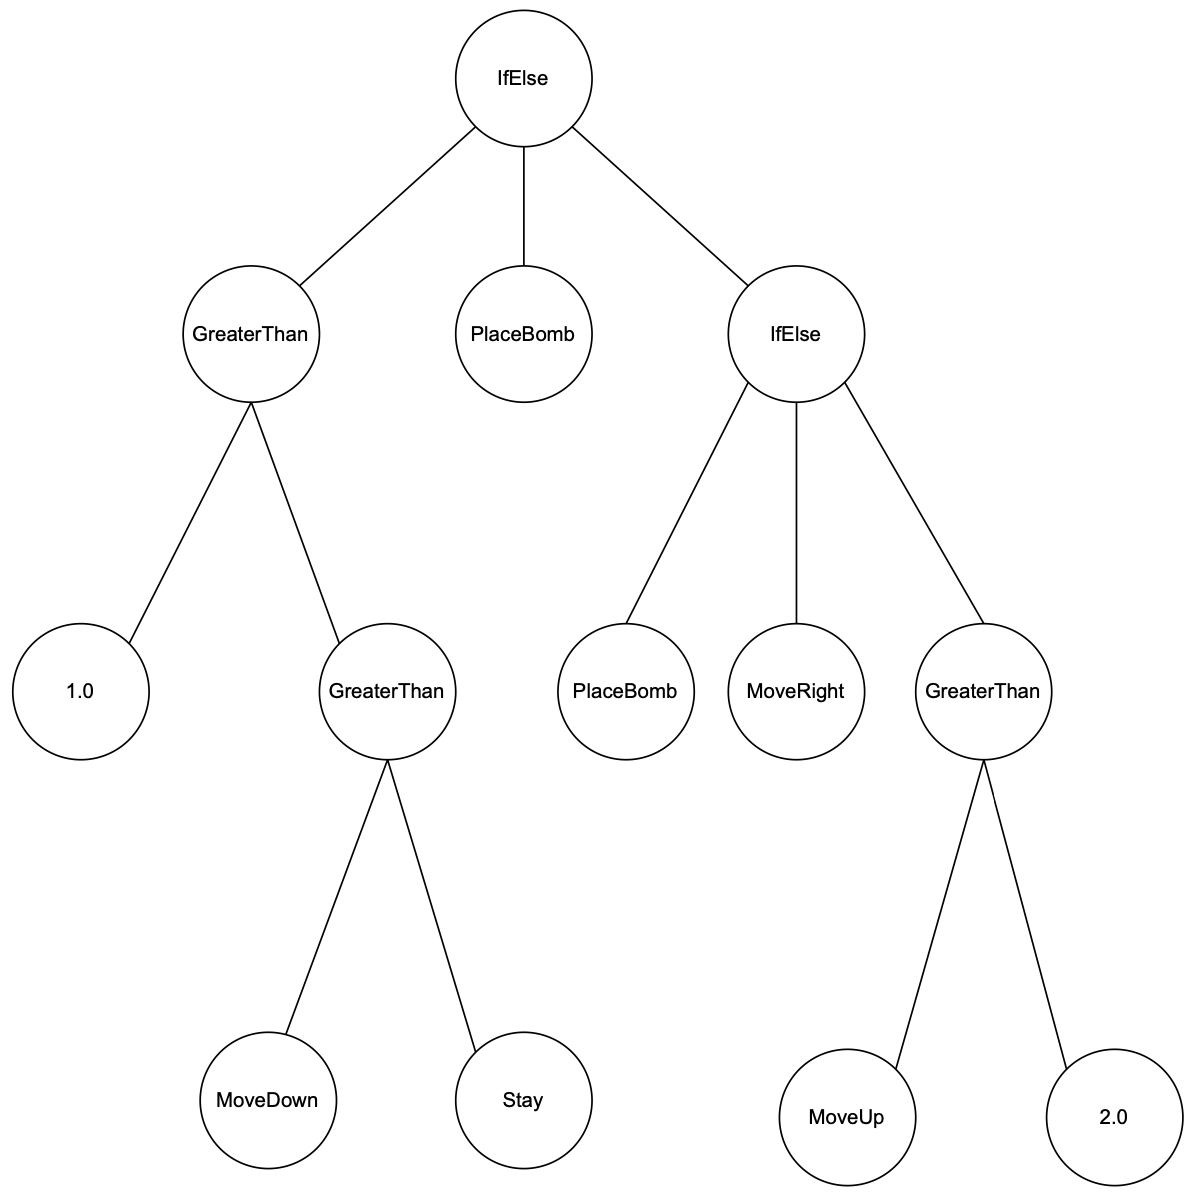
\includegraphics[width=0.7\linewidth]{pictures/treeWithDepthOfThree}
	\caption{}
	\label{fig:treewithdepthofthree}
\end{figure}

The evolutionary algorithm chosen for the second implementation is tree-based genetic programming (GP). This approach offers multiple benefits: 

\begin{enumerate}
	\item First, it is highly flexible. The tree structure allows a wide range of programs to be represented by the algorithm. 
 	\item Furthermore, GP can \cite{TreeBasedGPWeb}"discover novel and unexpected solutions that may not be apparent to human programmers,"  as the algorithm is not biased toward favoring certain approaches over others, as long as they are within the rules set by the programmer or hardware.
  	\item Additionally, GP can easily adapt to changing requirements and inputs, making it highly adaptable.
  \end{enumerate}
This approach was chosen due to its high flexibility. While the initial training phase against the already implemented AI players might be more challenging due to the complexity of the setup compared to other algorithms like Differential Evolution or regular Genetic Algorithms, the benefits of flexibility and adaptability to new circumstances are promising in an environment where multiple evolutionary algorithms compete against each other. 

\subsection{Design Decisions}

The implementation of the algorithm is encapsulated in the GeneticPlayer class. This class does not inherit from the AIPlayer class, which already contains significant functionality. Inheritance was avoided because the setup of genetic programming differs significantly from "regular" genetic algorithms. GP uses a tree structure and consists of multiple components (functions, terminals, and constants). Terminals represent the leaf nodes of the tree, whereas functions branch out, increasing the complexity of the tree. \\ 
The GeneticPlayer class contains an abstract static class called Operation, which serves as the base for all terminals and functions. The respective terminals and functions inherit from Operation. The terminals include basic movement operators such as MoveUp, MoveDown, MoveLeft, MoveRight, and Stay, which represent movements in the game along the x- and y-axes. Additional terminals include IsTargetZone, CheckForBomb, PlaceBomb, CheckForExtra, GetDistanceToEnemy, and three constant values. These terminals encapsulate functionality already implemented for the AIPlayer, allowing the GP to iterate over it. The constant values are arbitrary defaults that can be adjusted based on the algorithm's performance or goals.

The algorithm also relies on two operations: GreaterThan and IfElse. GreaterThan has an arity of 2, meaning it compares two values, returning 1 if the first value is greater than the second and 0 otherwise. IfElse has an arity of 3. It checks whether the first value is greater than 0. If true, it forwards the value t[1]; otherwise, it forwards t[2].


In the picture above one can see a possible scenario of a tree being built. The functions can never represent leave nodes. They always have multiple nodes attached to them below. The terminals on the other hand represent leave nodes and therefore no longer branch out. 

The core of the GP is the initializeGP method. In this method, functions and terminals are initialized, and the maximum tree depth is set. During the training phase, a depth of 5 was used, but this can be adjusted based on performance. Poli et al. (2008) suggest that \cite{poli2008fieldguide} "the choice of tree depth and operator arity significantly impacts the complexity and performance of genetic programs, guiding our decision to use a tree depth of 5." 

The engine combines the algorithm's constraints with the fitness function. Parameters such as population size, mutation rate, and crossover rate can be manually adjusted depending on the algorithm's performance. The result performs the actual training by streaming the data and applying the constraint of the number of generations. Finally, the best strategy is returned. \\ 
The fitness function is where the actual training occurs. Each time the fitness function is called, a new game and playground are initialized. A new GeneticPlayer and three new AIPlayer instances are created. Notably, during the training phase, a specific method, addAIForFitness, was implemented in the Game class. This method does not start the threads typically used during a game simulation.

The operations and terminals are linked to the newly created GeneticPlayer. 

\begin{lstlisting}[language=Java]
for (int i = 0; i < 1000; i++) {
    if (!game.isRunning() || goodboy.isDead()) {
        System.err.println("Fitness: Stopped at iteration " + i +
            ", game running = " + game.isRunning() +
            ", GoodBoy dead = " + goodboy.isDead());
        steps = i;
        break;
    }
    for (Player player : game.getPlayers()) {
        if (player instanceof AIPlayer aip) {
            System.err.println("Fitness: AIPlayer " +
                aip.getNickname() + " tick");
            aip.tick();
        } else {
            GeneticPlayer gp = (GeneticPlayer) player;
            double result = gp.program.eval();
            System.err.println("Fitness: GeneticPlayer tick, result = " +
                result + ", position = (" + gp.gridX + "," + gp.gridY + ")");
            if (result == 1.0 || result == 2.0 ||
                result == 3.0 || result == 4.0) {
                successfulMoves++;
            }
        }
    }
    game.tick();
}
\end{lstlisting}

In the loop, the player performs a maximum of 1,000 iterations before being forced to terminate. \\ 
The loop is interrupted if the player dies or the game is no longer running, simulating a real environment where the GP interacts with AIPlayer instances. In each iteration, both the AIPlayer and GeneticPlayer call their tickmethods, selecting a new action and synchronizing their current state. \\ 
After all players have synchronized, the game synchronizes with game.tick. During game.tick, selected bombs detonate, extras collected by players in the previous period modify their bomb range or capacity, and players may be killed by exploding bombs and removed from the game. Successful moves by the GP are recorded during the loop, as they impact the overall fitness.

The fitness function consists of multiple components: 
\begin{itemize}
      \item survivalTime 
      \item extrasCollected 
      \item deathPenalty 
      \item moveReward 
\end{itemize}

Since the algorithm aims to minimize the fitness function, beneficial actions for the GP receive a negative multiplier, while harmful actions receive a positive multiplier. Notably, the fitness function currently ignores the number of opponents the GP kills, meaning aggressive behavior does not affect fitness. \\
This design choice promotes defensive behavior, prioritizing survival over aggression. The goal is for the player to survive as long as possible, leading to longer games compared to aggressive strategies where the player either dies or kills quickly. This defensive approach, inspired by strategic games like chess where top players prioritize avoiding mistakes over attacking, is reinforced by a high deathPenalty and a strong emphasis on survivalTime as a negative metric.

The GeneticPlayer class also includes a tick method, called by the GeneticPlayerThread, which is started in a real game environment to visually observe the player's behavior. 

\subsection{Issues}
The algorithm in its current form does not perform as intended. Several issues arose during implementation, some of which remain unresolved: 
\begin{enumerate}
      \item Not inheriting from the AIPlayer class. 
      The primary issue, likely causing subsequent problems, was the decision not to inherit from the AIPlayerclass. Although this was a deliberate choice initially, it likely caused more harm than good. Much of the functionality was copied with slight adjustments, adding redundant code without significant value. The GeneticPlayer inherits from the Player class, sharing many variables with AIPlayer. \\ 
This required moving some code, such as the die and isDead methods, from AIPlayer to Player to make it accessible to the GP.
      \item Adjusting classes that were already functional. 
      Other classes, such as the Game class, were modified to include the tick method, which synchronizes player actions within a time frame. However, these adjustments introduced additional issues, complicating debugging. 
	  
	During the project, console output showed that the player performed actions like moving up and down, which sometimes succeeded and sometimes failed depending on obstacles like walls. However, the player never placed bombs. Debug print statements revealed that the condition player.bombs.size() < player.bombCount was never true, indicating that bombs always contained a bomb before the output statement was triggered. This led to replacing many System.out.println() statements with System.err.println(), suspecting that threading issues were affecting the print statements (as threads were initially started for all AIPlayer instances). 
 
 This hypothesis was confirmed, revealing another issue: the players and bombs were not synchronized.
      \item Synchronization of player behavior. 
      While AIPlayer instances were bound to a tick every 300 ms, bombs exploded every 4,000 ms. The GP, however, was not constrained by these timings, operating only limited by CPU capacity. This caused the GP to perform significantly more iterations before a bomb exploded, leading to poor assumptions about its behavior after placing a bomb, often resulting in the player committing suicide. Luke (2013) highlights the importance of \cite{Luke2013Metaheuristics} "synchronization in simulation-based evolutionary algorithms, which posed a significant challenge in aligning the tick rates of players and bombs in our implementation." \\ 
	  Ultimately, AIPlayer threads were disabled to remove artificial constraints designed for a realistic gaming experience, allowing the simulation to run without being bound by these limitations. 
   
   The above issues have left the algorithm only partially functional. Synchronization of triggered behaviors (bomb explosions, AIPlayer actions, and GeneticPlayer actions) caused significant problems. Many issues could have likely been avoided by inheriting most behavior from AIPlayer. The synchronization problem could have been mitigated by aligning the GP's tick time with that of the AIPlayer. However, this would have slowed the algorithm or reduced its quality, as the complexity and population size would need to be significantly reduced to maintain performance. 
\end{enumerate}

\section{Conclusion and Outlook}

\subsection{Team Reflection}
We couldn’t reach our initial goal where we wanted to implement 3 different algorithms and let them compete against each other. The only successful implementation was the differential evolution which was implemented by Sara.

Overall there were a couple of things we could potentially do better in any future projects:

Have more discussions about how the algorithms are implemented: While we had a good communication within the team and helped each other out as much as we could and asked from one another, we didn’t talk too much about how the respective algorithms are implemented. Some issues like the synchronization issue with the tree-based genetic algorithm could have been avoided since the DE was inheriting the AIPlayer.

\subsection{Evolutionary Training: Reflections and Next Steps}
For the evolutionary training component specifically, several insights emerged that could guide future work. Our implementation timeline proved challenging, as project specification uncertainties and concurrent academic commitments (including laboratory work and exams during the final month) delayed development. Starting implementation 2-3 months earlier would have provided sufficient time to fully realize our approach.

We also underestimated the integration complexity between the evolutionary training agent and other system components. This prevented the planned tournament-based evaluation against other agents, which was a key objective for comparative analysis.

Despite these challenges, the project yielded valuable insights:
\begin{itemize}
	\item Practical applications of data augmentation techniques
	\item Implementation considerations for Elo systems in AI evaluation
	\item Hands-on experience with the Jenetics framework
\end{itemize}

For future work on this specific component, we recommend:
\begin{itemize}
	\item Completing the agent implementation pipeline
	\item Executing systematic tournaments using our Elo framework
	\item Conducting cross-team agent competitions
\end{itemize}

\section{Author Contributions}
The work presented in this report represents a collaborative effort. Individual contributions to specific sections are detailed below:
\textbf{Widmann Lukas}: Section \ref{sec:tree_train} "Tree-Based Genetic Programming"
\newline \textbf{Dogà Sara}: Section \ref{de_train} "Fine-tuning Agent Behavior with Differential Evolution"
\newline \textbf{Askar Sami}: \newline
Section \ref{sec:evo_train} "Evolutionary Training with Human Data and Jenetics" 
\newline Maintained project repository and set up GitHub workflow \cite{rmb_github}
\newline Figure \ref{fig:possibleActionsPlayer}, Figure \ref{fig:workflow}

	 \textbf{Joint Work}: Introduction by mostly Dogà Sara with additions from Askar Sami;
	 
	  Conclusion and Outlook Team reflection: Mostly Lukas Widman with additions from Askar Sami


\bibliographystyle{alpha}
\bibliography{sample}
\end{document}
